\documentclass[11pt]{article}

\usepackage[utf8]{inputenc}
\usepackage[english]{babel}

\usepackage{hyperref}		  % For \autoref
\usepackage{parskip}		  % Don't indent paragraphs; skip instead.

\usepackage{amsfonts, amsmath, amssymb}
\usepackage{amsthm}
\usepackage{changepage} 	% For adjustwidth environment
\usepackage{colortbl}  		% Provides the  \arrayrulecolor command.
\usepackage{environ}
\usepackage{framed}			  % For leftbar environment
\usepackage{mathtools}		% For the \mathclap command.
\usepackage{ragged2e}		  % FlushLeft environment
\usepackage{thmtools}		  % For restatable environment
\usepackage{varwidth}
\usepackage{xcolor}
\usepackage{makeidx}
\usepackage{bm}           % For vector bold
\usepackage[margin=3cm]{geometry}


\newenvironment{indentone}{\begin{adjustwidth}{3em}{0em}}{\end{adjustwidth}}

% \renewcommand{\bfseries}{\scshape}
% \usepackage{ccfonts}
\newcommand\op[1]{{\ \mathrm{#1}\ }}
\newcommand\uop[1]{{\mathrm{#1}}}

\newcommand\AND{{\op{AND}}}
\newcommand\IMPLIES{{\op{IMPLIES}}}
\newcommand\MYS{{\op{MYS}}}
\newcommand\OR{{\op{OR}}}
\newcommand\NOT{{\uop{NOT}}}
\newcommand\XOR{{\op{XOR}}}
\newcommand\IFF{{\op{IFF}}}
\newcommand\VEC{\bm}{}
\newcommand\DIV{\>|\>}

\newcommand\FALSE{{\mathrm{F}}}
\newcommand\TRUE{{\mathrm{T}}}

% Number sets
\newcommand{\Nats}{\mathbb N}		% Naturals
\newcommand{\Ints}{\mathbb Z}		% Integers
\newcommand{\Q}{\mathbb Q}			% Rationals
\newcommand{\R}{\mathbb R}			% Reals
\newcommand{\C}{\mathbb C}			% Complexes
\newcommand{\cO}{\mathcal O}		% Big-Oh
\newcommand{\cP}{\mathcal P}		% Power set

\theoremstyle{definition}
\newtheorem{theorem}{Theorem}[section]
\newtheorem{corollary}{Corollary}[section]
\newtheorem{lemma}{Lemma}[section]
\newtheorem{proposition}{Proposition}[section]
\newtheorem{definition}{Definition}[section]
\newtheorem{remark}{Remark}[section]
\newtheorem{example}{Example}[section]
\newtheorem{question}{Question}[section]
\newtheorem{problem}{Problem}[section]
\newtheorem{exercise}{Exercise}[section]
\newtheorem{homework}{Homework}[section]
\newtheorem{algorithm}{Algorithm}[section]
\numberwithin{equation}{section}
% \newtheorem*{corollary}{Corollary}
% \newtheorem*{theorem}{Theorem}
% \newtheorem*{definition}{Definition}
% \newtheorem*{remark}{Remark}


% Essential sections of notes, e.g. definitions/theorems.
\NewEnviron{bigbox}{{

    \newdimen\slidewidth
    \slidewidth=\linewidth
    % Without this, I get errors beginning "Overfull \hbox (6.79999pt too
    % wide)"
    \advance\slidewidth by -7pt

    \medskip

    \fbox{parbox{\slidewidth}{\BODY}}

    \medskip

  }}

% Stuff I should write or draw during lecture. (from James)
% Additional notes


\NewEnviron{writenotes}{\vspace{1ex}\begin{leftbar}{\BODY}\end{leftbar}}

\title{Notes\\
  {\large STA302H1 - Fall 2020}}
\author{Ziyue Yang}

\begin{document}
\maketitle

\tableofcontents

\newpage

\section{Module 1 - Introduction to Data Analysis}

% \subsection{Introduction to Analyzing Data}

% \begin{definition}
%   Data is a collection of numbers, characters, images, or other items that provide information about something. (\textit{SDM, 3rd CE, DeVeaux et al})
% \end{definition}

% \textbf{How to organize raw data}

% A data file: cases and variables.

% \textbf{Types of Variables}

% All variables: Numerical: Continuous, Discrete; Categorical: Nominal (Unordered categorical), Ordinal (ordered categorical)

\subsection{What is SLR?}

\subsubsection{Basic Concepts of a Regression Model}

A regression model is a tendency of the response variable $Y$ to vary with the predictor $X$ in a systematic fashion. It's usually a scattering of points around the curve of statistical relationship.

There is a probability distribution of $Y$ for each level of $X$. The means of these probability distributions vary in some systematic fashion with $X$.



\newpage

\section{Module 2 - The SLR Model}

\subsection{What is a Linear Model?}

\begin{definition}[General Form of Models]
  General form of a model for $Y$ in terms of three predictors:
  \begin{equation}
    Y = f(X_1, X_2, X_3) + e
  \end{equation}
  \begin{itemize}
    \item $f$ is some unknown function
    \item $e$ is the error not accounted for $f$
  \end{itemize}
\end{definition}
  \begin{writenotes}
    Notice there issue here: if $f$ is a smooth, continuous function, then there are many possibilities for $f$. Also, we would need infinite data to estimate $f$ directly.

    A solution is to restrict $f$ to a \textit{linear form}.
  \end{writenotes}

\begin{definition}[Linear Model]
  In a linear model for $Y$, the \textit{parameters enter linearly} or $Y$ \textit{is linear in terms of the parameters}.
\end{definition}

\begin{example}
Here are some examples of linear models
\begin{align}
  Y &= \beta_0 + \beta_1 x + e\\
  Y &= \beta_0 + \beta_1\log(x) + e\\
  Y &= \beta_0 + \beta_1 x + \beta_2 x^2 + e\\
  Y &= \beta_0 + \beta_1\log(x_2) + \beta_2 x_2 + \beta_3 x_1 x_2 + e\\
  Y &= \beta_0 x^{\beta_1}e\label{linear-example-1}\\
  Y &= \exp(\beta_0 + \beta_1x + e)
\end{align}

\end{example}
\begin{writenotes}
  Tip: apply suitable transformations to $Y$ to see that the model is linear.

  Take (\ref{linear-example-1}) as an example, we can perform a log-transformation such that
  \begin{equation}
     \log(Y) = \log(\beta_0) + \beta_1\log(x) + \log(e)
  \end{equation}
\end{writenotes}

\begin{example}
  Here are some examples of non-linear models
  \begin{align}
    Y &= \beta_0 + \exp(\beta_1 x) + e\\
    Y &= \exp(\beta_0 + \exp(\beta_1 x)) + e\\
    Y &= \beta_0 + \beta_1 x\beta_2 + e\\
    Y &= \beta_0 + \beta_1 x - \exp(\beta_2 + \beta_3 x) + e
  \end{align}
\end{example}

\subsubsection{Linear and Nonlinear Models}

True nonlinear models are rare. Linear models can handle complex datasets. Since predictors can be transformed and combined in many ways, lienar models are \textit{very flexible}.

Note that all straight lines are linear models, but all linear models are not just straight lines.

\subsection{Simple Linear Regression Models}

\begin{equation}
  Y = \beta_0 + \beta_1 X + e
\end{equation}
\begin{itemize}
\item $Y$ - dependent or response or output variable
\item $X$ - independent or explanatory or predictor or input variable
\item $\beta_0$ - intercept parameter
\item $\beta_1$ - slope parameter
\item $e$ - random error/noise, variation in measures that we cannot account for
\end{itemize}

\subsection{Estimating the Regression Parameters}

\textbf{Fitting an SLR Model}

We wish to fit the SLR model

\begin{equation}
 Y = \beta_0 + \beta_1 X + e
\end{equation}

Our aim is, given a specific value of $X$, i.e. $X = x$, find the expected value of $Y$,
\begin{equation}
  \mathbb{E}(Y\>|\>X = x)
\end{equation}

We need estimates of the regression parameters $\beta_0, \beta_1$, and we need to assess the fit.

Get data (observational or experimental):
\begin{indentone}
  $n$ pairs of bivariate data:
  \begin{equation}
    (x_1,y_1),(x_2,y_2),\dots(x_n,y_n)
  \end{equation}
\end{indentone}
  Notation:
  \begin{indentone}
    Estimators: $\hat{\beta_0},\hat{\beta_1}$

    Estimates: $b_0,b_1$
  \end{indentone}

\newpage

\textbf{Geometrical Representation of Estimating $\beta$}

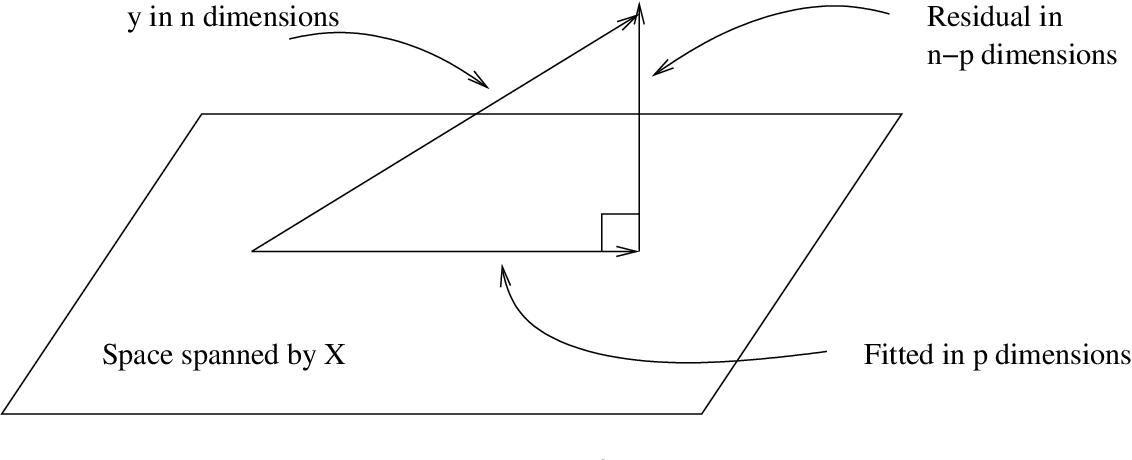
\includegraphics[scale = 0.4]{images/faraway-2005-2.1}

\begin{itemize}
  \item The response $Y$ is an $n$-dimensional space, $\VEC{Y}\in\R^n$
  \item The regression parameters are in a $p+1$-dimensional space, $\VEC{\beta}\in\R^{p+1}$, where $p$ is the number of predictors, so $p+1$ is the number of regression parameters: $p < n$.
\end{itemize}

\subsubsection{The Least Squares Method}


\begin{definition}[\textbf{Least Squares Method}]
Consider
\begin{equation}
  RSS = \sum^n_{i=1}[y_i - (b_0 + b_1x_i)]^2
\end{equation}

This is called the `least squares criterion'.

The \textbf{least squares method} aims to find the esitmators $b_0,b_1$ such that $RSS$ is minimized.

For each $x_i$, the predicted/fitted value is
\begin{equation}
  \hat{y_i} = b_0 + b_1x_i
\end{equation}

the residuals are 
\begin{equation}
  \hat{e_i} = y_i - \hat{y_i}
\end{equation}
\end{definition}

\begin{question}
  Why are we using vertical distances instead of horizontal distances?
\end{question}

We want to predict $Y$ from $X$ and so we want $\hat{y_i}$ to be as close as possible to $y_i$. 

Note that \textit{regression is not symmetric}. If we minimize the horizontal distances, we will get a different answer for $b_0$ and $b-1$. It matters which variable is dependent and which is independent.

\textbf{Why squared deviations?}
\begin{enumerate}
  \item Square deviations make NO satistical assumptions
  \item MSE is the most common way to measure error in statistics
  \item LS estimators have \textit{good} properties
\end{enumerate}

\begin{example}
  Often, raw deviation $\sum^n_{i=1}(y_i - \hat{y_i}) \equiv 0$.
\end{example}

\textbf{Analytical Derivations}

Consider the least square criterion

\begin{equation}
 RSS = \sum^n_{i=1}[y_i - (b_0 + b_1x_i)]^2
\end{equation}

Using calculus to minimize $RSS$, we get the normal equations:

wrt $b_0$:
\begin{align}
  \frac{\partial RSS}{\partial b_0} &= -\sum(y_i - b_0 - b_1x_i)\\
  &\stackrel{\text{set}}{=}0\\
  \implies \sum y_i &= \sum b_0 + \sum b_1x_i\\
  \implies n\bar{y} &= nb_0 + b_1n\bar{x}\\
  \implies b_0 &= \bar{y} - b_1\bar{x}\label{b_0-normal-equation}
\end{align}

wrt $b_1$:
\begin{align}
  \frac{\partial RSS}{\partial b_1} &= -2\sum^n_{i=1}(y_i - b_0 - b_1x_i)x_i\\
  &\stackrel{\text{set}}{=} 0\\
  \implies \sum x_iy_i &= \sum b_0x_i + \sum b_1x_i^2\\
  \implies \sum x_iy_i &= (\bar{y} - b_1\bar{x})\sum x_i + b_1\sum x_i^2\qquad\text{substitute (\ref{b_0-normal-equation})}\\
  \implies b_1 &= \frac{\sum x_iy_i - n\bar{x}\bar{y}}{\sum x_i^2 - n\bar{x}^2}
\end{align}

Therefore the \textbf{normal equations} are

\begin{gather}
  \boxed{b_0 = \bar{y} - b_1\bar{x}}\\
  \boxed{b_1 = \frac{\sum x_iy_i - n\bar{x}\bar{y}}{\sum x_i^2 - n\bar{x}^2}}
\end{gather}

\subsubsection{The Maximum Likelihood Estimator (MLE)}

Parameter $\VEC{\theta}$, Estimator $\hat{\VEC{\theta}}_{MLE}$

Steps for MLE:

\begin{enumerate}
  \item Define the \textbf{likelihood function} as a function of the parameter(s) $\VEC{\theta}$:
  \begin{equation}
    \mathcal{L}(\VEC{\theta}) = Distribution(Y\>|\>\VEC{\theta})
  \end{equation}
  conseidered a working model of the parameter given the specific data
  \item Find the \textbf{value of the parameter that maximizes the likelihood function}; i.e. the estimator that gives the highest probability density to the observed data
  \begin{equation}
    \hat{\VEC{\theta}}_{MLE} = \arg\max_{\theta}\mathcal{L}(\VEC{\theta})
  \end{equation}
\end{enumerate}

\textbf{MLE Properties}
\begin{itemize}
  \item Regularity conditions are required to derive the asymptotic distribution of the MLE
  \item Inference follows the frequentist paradigm
  \item MLE's have nice properties:
  \begin{itemize}
    \item Asymptotically Unbiased
    \item Consistent
    \item Sufficient
    \item Have minimum variance
    \item Invariant principle holds
  \end{itemize}
\end{itemize}

\begin{example}
  Consider a normal likelihood for $Y$ interms of the parameters $\VEC{\beta}, \sigma^2$
  \begin{equation*}
    \mathcal{L}(\VEC{\beta},\sigma^2)\sim\mathcal{N}_n(\VEC{x\beta}, \sigma^2\VEC{I}_n)
  \end{equation*}

  Using calculus we get
  \begin{gather*}
    \hat{\beta}_{0,MLE},\hat{\beta}_{1,MLE}\text{ same as in LS method}\\
    \hat{\sigma}^2_{MLE}=\frac{\sum(y_i - \hat{y}_i^2)}{n}
  \end{gather*}
\end{example}

\newpage

\subsubsection{Bayesian Approach}

In the Bayesian method, the parameters are considered random - instead of fixed constants

\begin{equation*}
  p(\VEC{\beta}), p(\sigma^2)
\end{equation*}
\begin{enumerate}
  \item Therefore, the parameters have a \textbf{prior distribution}. Priors could be either \textit{proper} or \textit{improper} (check out STA261 notes for further details).
  \item Assume a \textbf{likelihood} for $Y$, as a function of the parameters
  \begin{equation*}
    \mathcal{L}(\VEC{beta}, \sigma^2) = Distribution(Y\>|\>\VEC{\beta,\sigma^2})
  \end{equation*}
  \item Derive the \textbf{posterior distribution} of the parameters given the data
  \begin{equation}\label{posterior-distribution}
    p(\VEC{\beta},\sigma^2\>|\>y) \propto \mathcal{L}(\VEC{\beta},\sigma^2)\times\pi(\VEC{\beta},\sigma^2)
  \end{equation}
\end{enumerate}

\begin{writenotes}
We obtain \textbf{credible} (rather than confidence) intervals for $\VEC{\beta}$. Note that the interpretation differs.

With a credible interval, we speak about the probability that the unknown parameter falls into the interval.

Computationally, the Bayesian approach is more challenging than the LS/ML approach.
\end{writenotes}

\begin{example} An example of Bayesian approach
  \begin{enumerate}
    \item Choose improper prior
    \begin{equation*}
      \pi(\VEC{\beta},\sigma^2)=p(\VEC{\beta})\times p(\sigma^2)\propto\sigma^2
    \end{equation*}
    \item Assume a likelihood for $Y$
    \begin{equation*}
      \mathcal{L}(\VEC{\beta},\sigma^2)\sim\mathcal{N}_n(\VEC{x\beta},\sigma^2\mathbf{I}_n)
    \end{equation*}
    \item The posterior distribution of $\VEC{\beta}$ given the data is the kernel of a $(k+1)$-dimensional $t$ distribution
  \end{enumerate}
  \begin{writenotes}
  
  \underline{Results}

  Posterior mean results are identical to the LS approach.

  Posterior mean results are identical to the ML approach \textit{under normality}.

  $100(1-\alpha)\%$ credible intervals yield the same results as the $100(1-\alpha)\%$ confidence intervals, though the interpretations are different.
  \end{writenotes}
\end{example}

\newpage
\subsection{Properties of Least-Square Estimators}
\subsubsection{Properties of the Fitted Line}

Intercept parameter estimate (\ref{b_0-normal-equation})
\begin{equation}
  b_0 = \bar{y} - b_1\bar{x}
\end{equation}

Slope parameter estimate
\begin{equation}\label{slope-estimate}
  b_1 = \frac{\sum^n_{i=1}x_iy_i - n\bar{x}\bar{y}}{\sum^n_{i=1} x^2 - n\bar{x}^2}=\frac{\sum^n_{i=1}(x_i-\bar{x})(y_i-\bar{y})}{\sum^n_{i=1}(x_i-\bar{x})^2}=\frac{SXY}{SXX}
\end{equation}

\begin{writenotes}
  \textit{Derivation of}~(\ref{slope-estimate}).

\underline{Numerator}
  \begin{align*}
    \sum(x_i - \bar{x})(y_i - \bar{y}) &= \sum(x_i - \bar{x})y_i - \sum(x_i - \bar{x})\bar{y}\\
    &= \sum(x_i - \bar{x})y_i - \bar{y}\sum(x_i - \bar{x})
  \end{align*}
  Note that $\sum(x_i - \bar{x})\equiv 0$, since
  \begin{align*}
  \sum x_i - \sum\bar{x}
    &= \sum{x_i} - n\bar{x}\\
    &= \sum x_i - n\left( \frac{\sum x_i}{n} \right) = 0
  \end{align*}

Same applies, $\sum(y_i - \bar{y}) \equiv 0$.

\underline{Denominator}
\begin{align*}
  \sum(x_i - \bar{x})^2 &= \sum(x_i - \bar{x})x_i - \sum(x_i - \bar{x})\bar{x}\\
  &= \sum x_i^2 - \bar{x}\sum x_i - \bar{x}\sum(x_i - \bar{x})\\
  &=\sum x_i^2 - n\bar{x}^2\qquad\text{since }\sum x_i=n\bar{x}
\end{align*}
\end{writenotes}

\subsubsection{Interpreting Regression Parameter Estimates}

\underline{Slope, $b_1$}

When $x$ changes by $1$ unit, the corresponding average change in $y$ is the slope.

\underline{Intercept, $b_0$}

The average value of $y$ when $x = 0$. (No parctical interpretation unless $0$ is within the range of the predictor ($x$) values.)

\subsubsection{Properties of Fitted LS Regression Line}

Consider a fitted line

\begin{equation*}
  \hat{y} = b_0 + b_1 x
\end{equation*}

\begin{enumerate}

\item The average of the residuals is always 0, i.e.

\begin{equation}\label{sum-residuals-zero}
  \sum^n_{i=1}\hat{e}_i \equiv 0
\end{equation}

\begin{proof}
\begin{align*}
  \sum (y_i - \hat{y}_i) &= \sum(y_i - b_0 - b_1x_i)\\
  &= \sum y_i - nb_0 - b_1\sum x_i\\
  &= n\bar{y} - n(\bar{y} - b_1\bar{x}) - b_1n\bar{x}\\
  &= 0
\end{align*}
\end{proof}

\item The Sum of Squares of Residuals is NOT $0$, \textit{unless the fit to the data is perfect}.

\begin{equation}\label{RSS-not-zero}
  RSS = \sum^n_{i=1}\hat{e}_i^2 \neq 0
\end{equation}

This criteria is a minimum as reqiuired by the LS method.

\item $\sum \hat{e}_ix_i = 0$
\item $\sum \hat{e}_i\hat{y}_i=0$
\item $\sum \hat{y}_i = \sum y_i$ (sum of fitted values $=$ sum of observed)
\end{enumerate}

\subsubsection{Gauss-Markov Theorem}

\begin{theorem}[Gauss-Markov Theorem]
  Under the conditions of the SLR model, the least-squares parameter estimators are BLUE (``Best Linear Unbiased Estimators'').
  \begin{itemize}
    \item Parameter $\theta$; Estimator $\hat{\theta}$
    \item Linear - linear in parameters
    \item Unbiased, $\mathbb{E}(\theta)$, i.e. does NOT overestimate or underestimate systematically
    \item ``Best'' - Obtain \textbf{minimum variance} among all unbiased linear estimators
  \end{itemize}
\end{theorem}

\subsubsection{Properties of Slope Estimator: Expectation}

Recall from~(\ref{slope-estimate}) that

\begin{equation}
b_1 = \frac{\sum^n_{i=1}x_iy_i - n\bar{x}\bar{y}}{\sum^n_{i=1} x^2 - n\bar{x}^2}=\frac{\sum^n_{i=1}(x_i-\bar{x})(y_i-\bar{y})}{\sum^n_{i=1}(x_i-\bar{x})^2}=\frac{SXY}{SXX}
\end{equation}

Since $\sum (x_i - \bar{x}) = 0$,

\begin{equation*}
\sum^n_{i = 1} (x_i - \bar{x})(y_i - \bar{y}) = \sum^n_{i = 1}(x_i\bar{x})y_i - \bar{y}\sum^n_{i = 1}(x_i - \bar{x}) = \sum^n_{i=1}(x_i-\bar{x})y_i
\end{equation*}

Let $c_i = \frac{x_i - \bar{x}}{SXX}$, then rewrite $b_1$ as
\begin{equation}
  \boxed{b_1 = \sum^n_{9 = 1}c_iy_i}
\end{equation}

Treat $X$'s as fixed, the the mean of slope estimate, $b_1$, is

\begin{align*}
  \mathbb{E}(b_1\>|\> X) &= \mathbb{E}\left[ \sum^n_{i = 1} c_iy_i\>|\> X = x_i\right]\\
  &= \sum c_i\mathbb{E}(y_i\>|\> X = x_i)\\
  &= \sum c_i (\beta_0 + \beta_1x_i)\\
  &= \beta_0\sum c_i + \beta_1\sum c_ix_i,
\end{align*}

Note that
\begin{enumerate}
\item $\sum c_i = \sum(x_i-\bar{x}) / SXX = 0$
\item $\sum c_ix_i=\sum(x_i - \bar{x}) x_i / SXX = SXX / SXX = 1$
\end{enumerate}

\begin{equation}\label{b_1-unbiased}
  \implies \boxed{\mathbb{E}(b_1\>|\> X) = \beta_1}\qquad\text{ i.e. $b_1$ is unbiased.}
\end{equation}

\subsubsection{Properties of Intercept Estimator: Expectation}

Recall that $b_0 = \bar{y} - b_1\bar{x}$

Mean of intercept estimate, $b_0$

\begin{align*}
  \mathbb{E}(b_0\>|\>X) &= \mathbb{E}[(\bar{y} - b_1\bar{x})\> X = x_i]\\
  &= \mathbb{E}(\bar{y}\>|\>X = x_i) - \bar{x}\mathbb{E}(b_1\>|\>X = x_i)\\
  &= \mathbb{E}\left( \frac{\sum y_i}{n} \>|\> X = x_i \right) -k \bar{x}\beta_1\\
  &= \frac{1}{n}\sum\mathbb{E}(y_i \>|\> X=  x_i) - \bar{x}\beta_1\\
  &= \frac{1}{n}\sum(\beta_0+\beta_1x_i) - \bar{x}\beta_1\\
  &= \frac{1}{n}(n\beta_0 + \beta_1\sum x_i) - \bar{x}\beta_1\\
  &= \beta_0 + \beta_1\frac{n\bar{x}}{n} - \bar{x}\beta_1\\
  &= \beta_0
\end{align*}

Hence $b_0$ is unbiased for $\beta_0$.

\subsubsection{Properties of Slope Estimator: Variance}

Variance of slope estimate, $b_1$

\begin{align}
  Var(b_1\>|\>X) &= Var\left[ \sum^n_{i=1}c_iy_i \>|\> X = x_i \right]\\
  &= \sum c_i^2Var(y_i\>|\>X = x_i)\\
  &= \sum c_i^2\sigma^2\\
  &= \sigma^2 \sum c_i^2\\
  &=\sigma^2\sum\frac{(x_i - \bar{x})^2}{(SXX)^2}\\
  &= \sigma^2\frac{SXX}{(SXX)^2}\\
  &= \frac{\sigma^2}{SXX}
\end{align}

\subsubsection{Properties of Intercept Estimator: Variance}

Vairance of intercept estimate, $b_0$

\begin{align}
  Var(b_0\>|\> X) &= Var[(\bar{y} - b_1\bar{x})\>|\> X = x_i]\\
  &= Var(\bar{y}\>|\> X = x_i) + Var(b_1\bar{x}\>|\>X = x_i) - 2Cov[(\bar{y},b_1\bar{x})\>|\> X=  x_i]\\
  &= \frac{\sigma^2}{n}+ \bar{x}^2\left( \frac{\sigma^2}{SXX} \right) - 2\bar{x}Cov\left[ \left(\frac{1}{n}\sum y_i,\sum c_iy_i\right)\>|\>X = x_i \right]\\
  &= \frac{\sigma^2}{n}+ \bar{x}^2\left( \frac{\sigma^2}{SXX} \right) - 2\frac{\bar{x}}{n}Cov\left[ \left(y_i,y_i\right)\>|\>X = x_i \right]\\
  &= \frac{\sigma^2}{n} + \frac{\bar{x}\sigma^2}{SXX} - \frac{2\bar{x}}{n}\sum c_i Var(y_i\>|\> X = x_i)\\
  &= \frac{\sigma^2}{n} + \frac{\bar{x}\sigma^2}{SXX} - 2\frac{\bar{x}}{n}\sigma^2\sum c_i\\
  &= \sigma^2\left(\frac{1}{n} + \frac{\bar{x}^2}{SXX}\right)
\end{align}

\subsection{Statistical Assumptions of SLR}
\subsubsection{SLR Assumptions}

\begin{enumerate}
  \item We assumed that $Y$ is related to $x$ by the SLR model
  \begin{gather*}
    Y_i = \beta_0 + \beta_1 x_i + e_i,\quad i = 1\dots n\\
    \OR\\
    \mathbb{E}(Y\>|\>X=x_i) = \beta_0 + \beta_1x_i
  \end{gather*}
  In other words, \textbf{the linear model is appropriate}.

  And the following three Gauss-Markov Conditions:
  \item \textbf{The errors have mean of 0}, i.e., 
  \begin{equation*}
    \mathbb{E}(e_i) = 0\quad i=1\dots n
  \end{equation*}
  \item \textbf{The errors have a common variance $\sigma^2$}, i.e.
  \begin{equation*}
    Var(e_i) = \sigma^2\quad i=1\dots n
  \end{equation*}
  Meaning the variation is the same for all observations, i.e. \textbf{homoscedastic}.
  \item \textbf{The errors are uncorrelated}, i.e. 
  \begin{equation*}
    Cov(e_i,e_j) = 0\quad \forall i\neq j
  \end{equation*}
\end{enumerate}

\subsubsection{Estimating Variance of Random Error Term}

The random error $e_i$ has mean $0$ and variance $\sigma^2$. The parameter $\sigma^2$ is another parameter of the SLR model. 

Our goal is to estimate $\sigma^2$, in order to measure the variability of our estimates of $Y$ and carry out inference on our model.

Notice that
\begin{equation}
  e_i = Y_i - (\beta_0 + \beta_1x_i) = Y_i - \text{unknown regression line at }x_i
\end{equation}
Replacing  $\beta_0,\beta_1$ by their LS estimates, we estimate the errors by
\begin{equation}
  \hat{e}_i = Y - (b_0 + b_1 x_i) = Y_i - \text{unknown regression line at }x_i
\end{equation}
Using the estimated errors, we can show that an \textit{unbiased} estimate of $\sigma^2$ is
\begin{equation}
  \boxed{S^2 = \frac{\sum \hat{e}_i^2}{n-2} = \frac{RSS}{n-2}}
\end{equation}

\subsubsection{Statistical Assumption for Inference}

\textbf{In order to make inferences}, we need one more assumption about the errors, $e_i$'s.

Assume that \textbf{the errors are Normally distributed},
\begin{gather*}
e_i\sim \mathcal{N}(0,\sigma^2)\\
\OR\\
  \VEC{e}\sim\mathcal{N}_n(0,\sigma^2\VEC{I}_n)
\end{gather*}

$\star$\textbf{\underline{Implications}}
\begin{enumerate}
  \item The Normality assumption implies that the errors are independent (since they are uncorrelated).
  \item Since $y_i = \beta_0 + \beta_1x_i + e_i$, $Y_i\>|\>x_i$ is normally distributed.
  \item The LS estimates of $\beta_0$ and $\beta_1$ are equivalent to their MLE's.
\end{enumerate}

\subsubsection{Sampling Distributions of Slope and Intercept Estimators}

Slope: Since $b_1=\sum c_iy_i$ is a lincomb of the $y_i$'s, $b_1\>|\>x$ is also normally distributed, i.e. 
\begin{equation}
  \hat{\beta}_1 = \mathcal{N}\left( \beta_1,\frac{\sigma^2}{SXX} \right)
\end{equation}

Intercept: Since $b_1\>|\> X$ is normally distributed, $\bar{y}$ is normally distributed and $b_0/x$ is a lincomb of $b_1\>|\>X$ and $\bar{y}$, we have that
\begin{equation}
  \hat{\beta_0}\sim\mathcal{N}\left[ \beta_0, \sigma^2\left( \frac{1}{n} + \frac{\bar{x}^2}{SXX} \right) \right]
\end{equation}

\newpage
\section{Module 3 - Theory and Inference for SLR I}

\subsection{Mean and Variance of a Sample Mean}
\begin{definition}[The Sample Mean]
  Let $Y_1\dots Y_n$ be a random sample of size $n$ from a population. Then the sample mean is defined as 
  \begin{equation}
    \bar{Y}=\frac{1}{n}\sum^n_{i=1} Y_i
  \end{equation}

\underline{Mean of $\bar{Y}$}:
  \begin{align}
    \mathbb{E}\left( \frac{1}{n}\sum^n_{i=1}y_i \right) &= \frac{1}{n}\mathbb{E}\left(\sum Y_i\right)\\
    &= \frac{1}{n}\sum\left( \mathbb{E}(Y_i) \right)\\ 
    &= \frac{1}{n}\sum \mu\\
    &= \frac{n\mu}{n}=\mu
  \end{align}

\underline{Variance of $\bar{Y}$}:
\begin{align}
  Var\left(\frac{1}{n}\sum Y_i\right) &= \left(\frac{1}{n}\right)^2 Var\left( \sum Y_i \right)\\
  &= \left(\frac{1}{n}\right)^2\sum Var( Y_i )\qquad\text{since }Y_i\text{'s iid}\\
  &= \frac{n\sigma^2}{n^2} = \frac{\sigma^2}{n}
\end{align}
\end{definition}

\begin{theorem}[Chi-Square Random Variable]
Let $Y_1\dots Y_n$ be a random sample of size $n$ from a normal distribution with mean $\mathbb{E}(Y_i) = \mu$ and variance $Var(Y_i)=\sigma^2$, and for $i=1\dots n$, define $Z_i$ by 
\begin{equation}
  Z_i=\frac{Y_i - \mu}{\sigma}
\end{equation}
Then $\sum Z_i^2$ has a $\chi^2$ distribution with $n$ degrees of freedom (df).
\end{theorem}
\begin{writenotes}
  In other words, the square of a standard normal random variable is a chi-square random variable with $1$ df.

  A lincomb of independent chi-square random variables leads to another chi-square random variable. We can use MGFs to show these properties.
\end{writenotes}

\begin{question}
  Suppose that $Y_1\dots Y_n$ is a random sample from a $\mathcal{N}(\mu,\sigma^2)$. Then for $s^2=frac{1}{n-1}\sum (Y_i - \bar{Y})^2$ (the sample variance), which distribution does the following term follow?
  \begin{equation*}
    \frac{(n-1)s^2}{\sigma^2}
  \end{equation*}
\end{question}
\begin{writenotes}
  $\mathbb{E}(s^2)=\sigma^2$, hence $\dots$
\end{writenotes}

\newpage
\section{Module 4 - Theory and Inference for SLR, Part II}
\subsection{Regression Analysis of Variance (ANOVA) Approach to Regression}
\textbf{Q.} How well does the regression line summarize the data?

(Figure here)

Notice that $Y_i - \bar{Y} = (\hat{Y}_i - \bar{Y}) + (Y_i - \hat{Y}_i)$. Squaring both sides yields
\begin{equation}
  (Y_i - \bar{Y})^2 = (\hat{Y}_i - \bar{Y})^2 + (Y_i - \hat{Y}_i)^2 + 2(\hat{Y}_i - \bar{Y})(Y_i - \hat{Y}_i)
\end{equation}

Now we define and derive $SST, SSReg, RSS$

\begin{align}
  SST = \sum^n_{i=1}(Y_i - \bar{Y})^2 &= \sum^n_{i=1}(\hat{Y}_i - \bar{Y})^2 + \sum^n_{i=1}(Y_i - \hat{Y}_i)^2 + 2\sum^n_{i=1}\hat{Y}_i(Y_i - \hat{Y}_i) + 2\sum^n_{i = 1}(Y_i - \bar{Y}_i)(-\bar{Y})\\
  &= \sum(\hat{Y}_i - \bar{Y})^2 + \sum (Y_i - \hat{Y}_i)^2 + 2\sum\hat{Y}_i\hat{e}_i - 2\bar{Y}
\end{align}
\begin{writenotes}
  Total Sum of Squares
\end{writenotes}

\begin{align}
  SSReg &= \sum^n_{i=1}(\hat{Y}_i - \bar{Y})^2\\
  &= b_1^2\sum^n_{i=1}(x_i - \bar{x})^2
\end{align}
\begin{writenotes}
  Model SS or Regression SS

  Amount of variation in $y$'s explained by regression line
\end{writenotes}

\begin{align}
  RSS &= \sum^n_{i=1}(Y_i - \hat{Y}_i)^2\\
  &= \sum^n_{i=1}\hat{e}_i^2
\end{align}
\begin{writenotes}
  Residual SS or Error SS

  Least square criterion

  Unexplained variation in $y$'s
\end{writenotes}

\textbf{Decomposition of Sums of Squares}
\begin{align}
  SST = \sum^n_{i=1}(Y_i - \bar{Y})^2 &= SSReg + RSS\\
  &= \sum^n_{i=1}(\hat{Y}_i - \bar{Y})^2 \sum^n_{i=1}(Y_i - \hat{Y_i})^2\\
  &= b_1^2\sum^n_{i=1}(x_i - \bar{x})^2 + \sum^n_{i=1}\hat{e}_i\\
  &= b_1^2SXX + RSS
\end{align}
\begin{writenotes}
  $\sum^n_{i=1}\hat{e}_i(x_i - \bar{x}) = 0$ since
  \begin{itemize}
    \item $\sum \hat{e}_i=0$
    \item $\sum \hat{e}_ix_i=0$
  \end{itemize}
\end{writenotes}

\begin{table}[h!]
\centering
 \begin{tabular}{||c c c c||} 
 \hline
 Source & SS & df & MS = SS/df \\ [0.5ex] 
 \hline\hline
 Regression Line & $SSReg = b_1^2SXX$ & $1$ & $\frac{b_1^2SXX}{1}$ \\
 Error & $RSS=\sum\hat{e}^2_i$ & $n-2$ & $\frac{\sum^n_{i=1}\hat{e}^2_i}{n-2} = S^2$ \\
 Total & $SST$ & $n-1$ &  \\ [1ex]
 \hline
 \end{tabular}
\end{table}

\subsubsection{The F-Distributions}

\begin{definition}
  Suppose $V$ and $W$ are independent random variables such that $V\sim\chi_\nu^2$ and $W\sim\chi_\omega^2$. Then
  \begin{equation}
    \frac{V/\nu}{W/\omega}\sim F(\nu,\omega)
  \end{equation}
\end{definition}

\begin{theorem}[Equivalent Test of $H_0:\beta_1=0$]

Under $H_0, \beta_1=0$,
\begin{equation}
  F_{obs} = \frac{MSReg}{MSE} = \frac{SSReg/1}{SSE/(n-2)}\sim F(1,n-2)
\end{equation}
% \begin{proof}
%   Recall that $MSReg = b_1^2SXX$ and $MSE = S^2$.

%   \textbf{OMIT for now}
% \end{proof}
\end{theorem}

\begin{theorem}
  Suppose $Q\sim T_\nu$. Then
  \begin{equation}
    Q^2\sim F(1,\nu)
  \end{equation}
\end{theorem}

\subsection{Connection Between Regression and Correlation Analysis}
\subsubsection{The Bivariate Normal Distribution}

\begin{definition}[Jointly Distributed]
  $X,Y$ are \textbf{jointly distributed} if their join density function is
  \begin{equation}
    f(x,y) = \frac{e^{-Q/2}}{2\pi\sigma_x\sigma_y\sqrt{1-\rho^2}},\qquad -\infty < x < \infty, -\infty < y < \infty
  \end{equation}
  where
  \begin{equation}
    Q = \frac{1}{1 - \rho^2}\left[ \frac{(x - \mu_x)^2}{\sigma_x^2} - 2\rho\frac{(x-\mu_x)(y-\mu_y)}{\sigma_x\sigma_y} + \frac{(y-\mu_y)^2}{\sigma_y^2}\right]
  \end{equation}
  and the \textbf{correlation between $X$ and $Y$} is
  \begin{equation}
    \rho = \frac{\mathbb{E}[(X - \mu_x)(Y - \mu_y)]}{\sqrt{\sigma_x^2\sigma_y^2}}
  \end{equation}
\end{definition}

\textbf{Properties of the Bivariate Normal Distribution}
\begin{itemize}
  \item The two \textbf{marginal} distributions are
  \begin{equation}
    X\sim\mathbb{N}(\mu_x,\sigma_x^2)\text{ and }Y\sim\mathcal{N}(\mu_y,\sigma_y^2)
  \end{equation}
  \item The \textbf{conditional} distribution of $Y$ given $X = x$ is
  \begin{equation}
    Y\>|\>X = x\sim\mathcal{N}\left( \mu_y + \rho\sigma^y\left(\frac{x - \mu_x}{\sigma_x}\right), (1-\rho^2)\sigma_y^2 \right)
  \end{equation}
  \item \textbf{Linear combinations} of $X$ and $Y$ are normally distributed.
  \item A zero covariance between $X$ and $Y$ implies that they are \textbf{statistically independent}. \textit{Note that this is not true in general for any two uncorrelated random variables.}
\end{itemize}

\subsubsection{Pearson's Sample Correlation Coefficient}
\begin{definition}
  If $X$ and $Y$ are random variables, \textit{a symmetric measure of the direction and strength of the linear dependence between them} is their \textbf{correlation}, $\rho$.

  Based on a sample of $n$ observed pairs $(x_i,y_i)$, the estimate of the population correlation, $\rho$ is \textbf{Pearson's Product-Moment Correlation Coefficient} $r$, formulated as
  \begin{equation}\label{XYcorrelation}
    r = \frac{\sum^n_{i}(x_i - \bar{x})(y_i - \bar{y})}{\sqrt{\sum^n_i(x_i - \bar{x})^2\sum^n_i(y_i - \bar{y})^2}}=\frac{SXY}{\sqrt{SXX\cdot SYY}}
  \end{equation}
\end{definition}
\begin{writenotes}
  It is the MLE of $\rho$, i.e. $\hat{\rho}_{MLE}=r$.
\end{writenotes}

\textbf{Facts about the Sample Correlation Coefficient}
\begin{itemize}
  \item It measures the \textbf{strength and direction of the linear relationship} between $X$ and $Y$
  \item It's \textbf{unit-free}
  \item Is always a member $\in[-1,1]$
  \begin{itemize}
    \item $r = 0$: no linear association
    \item $r = -1$: perfect negative linear relationship
    \item $r = 1$: perfect positive linear relationship
    \item The strength of the linear relationship increases as $r$ moves away from $0$
  \end{itemize}
\end{itemize}

\textit{Figure of scatterplots in Slides}

\subsubsection{Relationship between Regression and Correlation}
\begin{question}
  How is correlation linked to SLR?
\end{question}
\begin{writenotes}
  Symmetric relationship $Cov(X, Y) = Cov(Y, X)$

  In SLR, we
  \begin{itemize}
    \item Have a response
    \item Specify a predictor
    \item Estimate $\mathbb{E}(Y\>|\>X)$/predict $Y$
  \end{itemize}
\end{writenotes}

\begin{question}
  What if we test $H_0:\rho=0$?
\end{question}
\begin{writenotes}
  Involve $r$

  But how is this related to $H_0:\beta_1=0$?
\end{writenotes}

\subsubsection{Coefficient of Determination / R-Squared}
\begin{definition}[Properties and Interpretation of R-Squared]
  \begin{equation}\label{R-Squared}
    R^2 = \frac{\sum^n_i(\hat{Y}_i - \bar{Y})^2}{\sum^n_i(Y_i - \bar{Y})^2} = \frac{SSReg}{SST} = \frac{SST-RSS}{SST} = 1 - \frac{RSS}{SST}
  \end{equation}
\textit{Figure for Extreme Cases}
\begin{itemize}
  \item $R^2\in[0,1]$
  \item $R^2$ is NOT resistant to outliers, affected by the spacing of $X$.
  \item The higher the variation in $X$, the higher $R^2$ will be.
\end{itemize}
\end{definition}

\textbf{Use and Limitations of $R^2$}

$R^2$ gives the \textbf{percentage} of variation in $y$'s explained by regression line

A high $R^2$ does NOT indicate that the estimated regression line is a good fit. 
\begin{itemize}
  \item no absolute rules about how `big' it should be
  \item can get very high by \textit{overfitting}
\end{itemize}

$R^2$ is not meaningful for models without intercept.

To compare two models, $R^2$ is only useful if
\begin{enumerate}
  \item same observations, $y$'s in original units (not transformed)
  \item one set of predictor variables is a subset of the other
\end{enumerate}

\begin{theorem}
In SLR,
  \begin{equation}R^2 = r^2\end{equation}
\end{theorem}
\begin{proof}
  Recall from~(\ref{XYcorrelation}),~(\ref{R-Squared}) that
  \begin{gather*}
    r = \frac{\sum^n_{i}(x_i - \bar{x})(y_i - \bar{y})}{\sqrt{\sum^n_i(x_i - \bar{x})^2\sum^n_i(y_i - \bar{y})^2}}=\frac{SXY}{\sqrt{SXX\cdot SYY}} = \frac{SXY}{\sqrt{SXX\cdot SYY}}\\
    R^2 = \frac{\sum^n_i(\hat{Y}_i - \bar{Y})^2}{\sum^n_i(Y_i - \bar{Y})^2} = \frac{SSReg}{SST} = 1 - \frac{RSS}{SST} = \frac{b_1^2SXX}{SYY}
  \end{gather*}
  Hence 
  \begin{align*}
    b_1 = \frac{SXY}{SXX}, b_1^2 = \frac{(SXY)^2}{(SXX)^2} \implies R^2 &= \frac{SXY^2}{SXX^2}\cdot\frac{SXX}{SYY}\\ 
    &= \frac{SXY^2}{SXX\cdot SYY}\\
    &= r^2
  \end{align*}

\end{proof}

\subsubsection{Testing $H_0:\rho = 0$}

When the population is \textbf{bivariate normal} and we test
\begin{gather*}
  H_0:\rho_{XY} = 0,\\
  H_A:\rho_{XY} \neq 0.
\end{gather*}
It can be shown that the test statistic
\begin{equation}
  t_{obs} = \frac{r\sqrt{n - 2}}{\sqrt{1 - r^2}} = \frac{b_1}{\sqrt{\frac{S^2}{SXX}}}\sim T_{n-2}
\end{equation}
where $b_1$ corresponds to the slope estimate for the normal error SLR model.
\begin{writenotes}
  Equivalent to $H_0:\beta_1 = 0$

  Further, $b_1 = \frac{SXY}{SXX}\implies r = \frac{SXY}{\sqrt{SXX\cdot SYY}}$
\end{writenotes}

\subsection{Dummy Variable Regression}

Consider SLR where the predictor variable $X$ is categorical rather than quantitative.
\begin{itemize}
  \item Simplest case is when $X$ has only two levels
  \item Use a dummy or indicator variable for the two levels, i.e. takes on two values: $0$ or $1$ only
  \item The resulting regression model is used to test for the difference in two means
\end{itemize}

Regression model:
\begin{equation}
  \mu_{Y/x} = \beta_0 + \beta_1x
\end{equation}
Fitted Regression Line:
\begin{equation}
  \hat{y} = b_0 + b_1x
\end{equation}
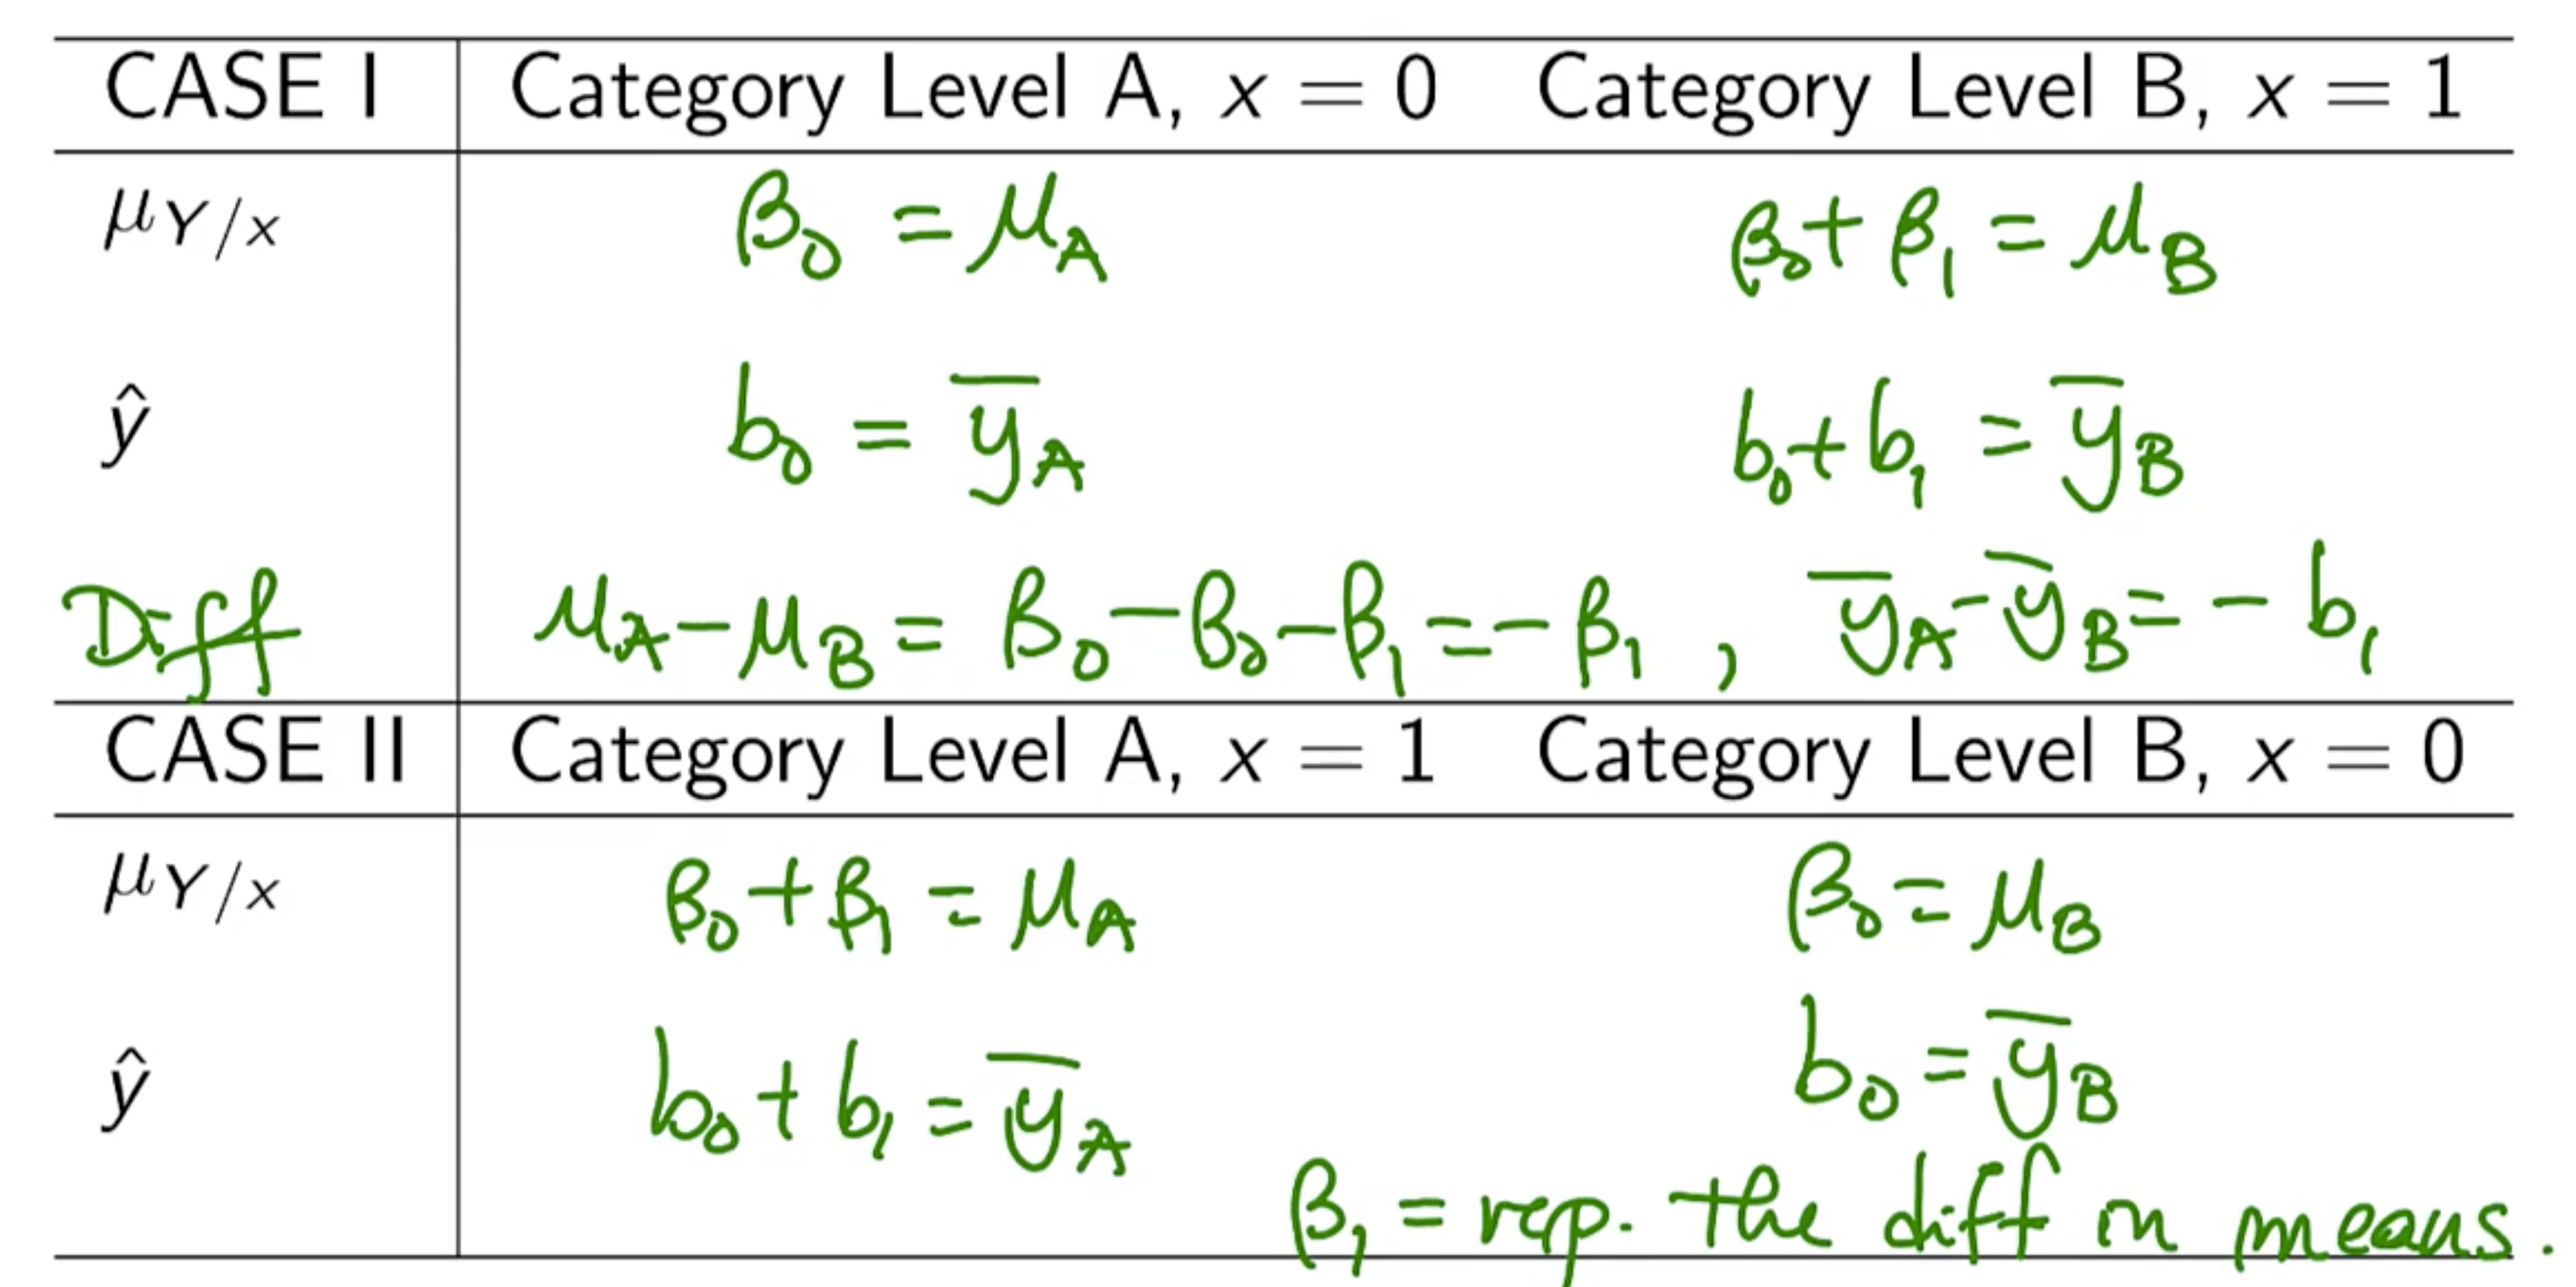
\includegraphics[width=\textwidth]{images/dummy-table}
\subsubsection{The Pooled Two-Sample $T$-Procedure}
Aim: Compare two independent populations means
\begin{equation*}
  H_0: \mu_A = \mu_B
\end{equation*}

Conditions:
\begin{itemize}
  \item Sampel 1: $A_1, A_2, \dots, A_n\stackrel{iid}{\sim}\mathcal{N}(\mu_A,\sigma_A^2)$
  \item Sample 2: $B_1, B_2, \dots, B_n\stackrel{iid}{\sim}\mathcal{N}(\mu_A,\sigma_A^2)$
  \item The two samples are independent
  \item The two populations have the same variance, i.e. $\sigma_A^2=\sigma_B^2=\sigma^2$
\end{itemize}

Test statistic:
\begin{equation*}
  t_{obs} = \frac{(\bar{A} - \bar{B}) - (\mu_A - \mu_B)}{s_p^2\sqrt{\frac{1}{n_A} + \frac{1}{n_B}}}\stackrel{H_0}{\sim}T_{n_A+n_B-2}
\end{equation*}
where $s_p^2=\frac{(n_A-1)s_A^2+(n_B-1)s_B^2}{n_A + n_B - 2}=\frac{\sum(n_i-1)s_i^2}{\sum(n_i-1)}$.

\begin{itemize}
  \item Population parameter: $\mu_a - \mu_B$
  \item Sample estimator: $\bar{A} - \bar{B}$
  \item Variance of sample estimator:
  \begin{align*}
    Var(\bar{A} - \bar{B})&= Var(\bar{A}) + Var(\bar{B})\qquad\text{since samples are independent}\\
    &=\frac{\sigma^2_A}{n_A} + \frac{\sigma^2_B}{n_B}\\
    &=\sigma^2\left(\frac{1}{n_A} + \frac{1}{n_B}\right)\qquad\text{since }\sigma_A^2=\sigma_B^2=\sigma^2.
  \end{align*}
  \item Pivotal Quantity:
  \begin{align*}
    \frac{(\bar{A} - \bar{B}) - (\mu_A - \mu_B)}{s_p^2\sqrt{\frac{1}{n_A} + \frac{1}{n_B}}} &= \frac{\frac{(\bar{A} - \bar{B}) - (\mu_A - \mu_B)}{\sigma^2\sqrt{\frac{1}{n_A} + \frac{1}{n_B}}}}{\sqrt{\frac{\sum(n_i - 1)\left[\frac{\sum(n_i-1)s_i^2}{\sum(n_i-1)}\left(\frac{1}{n_A} + \frac{1}{n_B}\right)\right]}{\sigma^2\left(\frac{1}{n_A} + \frac{1}{n_B}\right)\sum(n_i-1)}}}
  \end{align*}
  Note: $Z/\chi^2_{df/df}$.
\end{itemize}

\begin{example}[Pooled Two-Sample T Examples]
  \begin{enumerate}
    \item The difference between the average recovery times of an old and new drug.
    \item The difference in average condo price between downtown condos and uptown condos.
    \item The difference in mean length between Trout and Bass adult
    \item $\dots$
  \end{enumerate}
\end{example}

\subsection{Summary A: Data Analysis Tips}
\begin{enumerate}
  \item Is inference for:
  \begin{itemize}
    \item estimating a mean response,
    \item predicting a new observation or
    \item estimating the regression parameters
  \end{itemize}
  \item Do not extrapolate outside the data range of $X$
  \item The conditional bivariate Normal correlation model is equivalent to the Normal error SLR model.
  \item Correlation does not imply causation. Consider the context of the data, whether experimental or non-experimental.
  \item Statistical significance does NOT imply practical significance and vice versa.
\end{enumerate}

\newpage
\section{Module 5 - Diagnostics in SLR}
\subsection{Probability Plots}
Probability Plots are extremely useful tools to graphically assess goodness-of-fit. To see if the observed data follow a particular distribution, we plot the (observed) order statistics (from sorted data) against the (expected) theoretical quantiles (from a prob dist).

\textit{If the data follows the particular distribution, the plot should look roughly linear.}

The most common probability plot is the \textbf{Normal Q-Q plot}.

\textbf{The Shapiro-Wilk Test}
  \begin{enumerate}
    \item Null Hypotheses: The data follows a Normal Distribution
    \item Test Statistic: 
    \begin{equation*}
      W = \frac{(\sum_i^n a_ix(i))^2}{\sum^n_i (x_i - \bar{x})^2}
    \end{equation*}
    where
    \begin{itemize}
      \item $a_i = \frac{m'V^{-1}}{\sqrt{m'V^{-1}V^{-1}m}}$
      \item $m' = (m_1,\dots,m_n)$ are the expected values of standard normal order statistics
      \item $V$ is the covariance matrix of those normal order statistics
    \end{itemize}
    \item Decision Rule: If the $p$-value is less than the significance level, there is evidence that the data is \textbf{not Normal}.
  \end{enumerate}
\subsection{Properties of Residuals}
\begin{definition}[True Random Error]
Where $y_i = \mathbb{E}(y_i\>|\>X=x_i) + e_i = \beta_0+\beta_1x_i+e_i$, $e_i$ is the random fluctuation (or error) in $y_i$, i.e. 
\begin{equation}
  e_i = y_i - \mathbb{E}(y_i\>|\> X = x_i) = y_i - (\beta_0+\beta_1x_i)
\end{equation}
Under normal error SLR assumptions, we have that
\begin{equation}
  e_i\stackrel{iid}{\sim}\mathcal{N}(0,\sigma^2)
\end{equation}
\end{definition}

\begin{definition}[Estimated Errors/Residuals]
  \begin{equation}
    \hat{e}_i=y_i-\hat{y}_i=y_i-b_0-b_1x_i
  \end{equation}
\end{definition}

\textbf{Some Properties}
\textit{From the LS method}
\begin{enumerate}
  \item $\sum \hat{e}_i=0$
  \item $\sum \hat{e}_ix_i = 0$
  \item $\sum \hat{e}_i\hat{y}_i=0$
\end{enumerate}

\subsubsection{Mean and Variance of Residuals}

Expectation:
\begin{equation}
  \mathbb{E}(\hat{e}_i)=\mathbb{E}(y_i - \hat{y}_i) = \beta_0+\beta_1x_i-(\beta_0+\beta_1x_i)=0
\end{equation}

Variance:
\begin{equation}
  Var(\hat{e}_i) = (1-h_{ii})\sigma^2
\end{equation}

where $h$ is the \textbf{leverage}, defined as 
\begin{align}
  h_{ij} &= \frac{1}{n} + \frac{(x_i-\bar{x})(x_j-\bar{x})}{SXX},\quad\text{fix }i,j=1\dots n\\
  \implies i&=j,\quad h_{ij} =\frac{1}{n}+\frac{(x_i-\bar{x})^2}{SXX}\\
\end{align}

\begin{equation}
  \hat{y}_i=b_0+b_1x_i=\bar{y}-h\bar{x}+b_1x_i=\bar{y}+b_1(x_i-\bar{x})
\end{equation}

Recall $b_1=\sum_j(x_j-\bar{x})/SXX,\bar{y}=\sum y_j/n$, hence
\begin{align}
  \hat{y}_i&=\frac{\sum y_j}{n} + \frac{\sum(x_i-\bar{x})(x_j-\bar{x})}{SXX}y_j\\
  &= \sum^n_{j=1}h_{ij}y_j\\
  &= h_{ii}y_i+\sum_{j\neq i}h_{ij}y_j
\end{align}

\subsubsection{Covariance and Normality of Residuals}
Covariance:
\begin{equation}
  Cov(\hat{e}_i,\hat{e}_j)=-h_{ij}\sigma^2,\quad i\neq j
\end{equation}
Note: Residuals are NOT UNCORRELATED.

Normality:

\newpage
\section{Module 9 - Multiple Linear Regression Analysis}
\subsection{Review}
\textbf{Multiple Linear Regression (MLR)}
\begin{itemize}
\item MLR Model (to obtain using the least-squares estimation):
\begin{equation}
  \VEC{Y} = \VEC{X\beta} + \VEC{e},
\end{equation}
where
\begin{indentone}
$\VEC{Y}\in M_{n\times 1}$, 

$\VEC{X}\in M_{n\times(p+1)}$,

$\VEC{\beta}\in M_{p+1}$,

$\VEC{e}\in M_{n\times 1}$,

\end{indentone}

\item $p$ predictors: $p+1$ $\VEC{\beta}$'s
\item Gauss-Markov Conditions: $E(\VEC{e})=0, Var(\VEC{e})=\sigma^2 I$
\item Normal Error assumption (for inference)
\end{itemize}

\subsection{R-Squared and Adjusted R-Squared}

\begin{definition}[$R^2$: Coefficient of Multiple Determination]
  \begin{equation}
  R^2=\frac{SSReg}{SST}=1-\frac{RSS}{SST} = \frac{\VEC{Y'(H-\frac{1}{n} J)Y}}{\VEC{Y'(I-\frac{1}{n}J)Y}}
  \end{equation}

  called the coefficient of multiple determination (in the MLR setting).

  $R^2$ gives the percentage of variation in $Y$ explained by the model with all the $p$ predictors.
\end{definition}
\begin{writenotes}
  Note that it's NOT the square of a sample correlation coefficient ($r^2$) anymore.
\end{writenotes}

\begin{remark}
For the same $Y$, as $p$ increases, 

\begin{indentone}
  SST remains the same,

  SSReg stays the same or increases,

  RSS stays the same or decreases, 
\end{indentone}

hence $R^2$ either stays the same or increases.
\end{remark}

\begin{question}
  Is $R^2$ helpful in telling whether additional predictors are \textit{useful} for explaining the response?

  No.
\end{question}

\begin{definition}[Adjusted $R^2$]
  \begin{equation}
    R^2_{adj} = 1- \frac{RSS/(n-p-1)}{SST/(n-1)} = 1 - (n-1)\frac{MSE}{SST}
  \end{equation}

  where $S^2=\frac{RSS}{n-p-1}$ is an unbiased estimate of $\sigma^2=Var(e_i)=Var(Y_i)$.
  \begin{itemize}
    \item adjusted for the number of predictors in the model
    \item better to use instead of $R^2$
    \item always: $R^2_{adj} < R^2$ (note that the inequality is strict) 
  \end{itemize}
\end{definition}
\begin{writenotes}
  Case. $p > 1$ (MLR)
  \begin{indentone}
    Then $(n-1)/(n-p-1) > 1$
  \end{indentone}
  General case: as $p$ increases (adding more predictors to the model), $(n-1)/(n-p-1)$ increases.
\end{writenotes}

\subsection{Global and Partial F-tests}
\subsubsection{Motivational Examples: Salary vs. Experience, Wine Quality}
\begin{definition}[Global F-test]
  Testing Hypotheses: for $j=1\dots p$,
  \begin{gather}
    H_0: \beta_1=\beta_2=\dots=\beta_p=0\\
    H_a: \text{at least one } \beta_j \text{ is not } 0
  \end{gather}
  To test whether there is a linear association between $Y$ and all predictors.

  Test statistic:
  \begin{equation}
    F_{obs} = \frac{MSReg}{MSE}=\frac{SSReg/p}{RSS/(n-p-1)}
  \end{equation}

  Under $H_0$, $F_{obs}$ is an observation from the $F$ distribution with $df=(p,n-p-1)$.

  Hence we can conclude that
  \begin{indentone}
    Small p-value: Rhe model contains at least one significant predictor among the set of $p$ predictors

    Large p-value: None of the $p$ predictors are relevant for estimating/predicting $Y$.
  \end{indentone}
\end{definition}




\newpage

\section{Module 10 - Diagnostics in MLR}

\subsection{Inference for a Single Regression Coefficient}

\subsubsection{Hypothesis Testing}

As in SLR, we are interested in testing

\begin{equation}
  H_0: \beta_j = 0\text{ vs. }H_a: \beta_j\neq 0.
\end{equation}

Test statistic:

\begin{equation}
  t_{obs} = \frac{b_j}{SE(b_j)}
\end{equation}

Under $H_0$, $t_{obs}$ is an observation from the T distribution with $\text{df}=n-p-1$. This test gives an indication of whether or not the $j$th predictor, $X_j,j=1\dots p$, contributes to the prediction of the response variable \textbf{over and above} all the other predictors.

This is the special case of the Partial F-test with $k=1$

\subsubsection{Confidence Interval}

Confidence interval for $\beta_j, j=1\dots p$, assuming all the other predictors are in the model, is

\begin{equation}
  \beta_j \pm t_{\alpha/2, n-p-1}SE(b_j),
\end{equation}
(i.e. unbiased estimate $\pm$ Margin of Error, where MOE is the critical value $\times$ std error).

where
\begin{itemize}
  \item $b_j$: unbiased estimator of $\beta_j$
  \item $SE(b_j)$: standard error of the estimator
  \item $t_{\alpha/2, n-p-1}$: critical value of $100(1-\alpha/2)$th quantile from the T distribution with $\text{df}=n-p-1$.
\end{itemize}

\subsubsection{Global F-test vs. Individual t-tests}
\begin{itemize}
\item In SLR, these tests are equivalent
\item In MLR, the global F-test is designed to test the \textit{overall model}, while the $t$-tests are designed to test \textit{individual coefficients}.
\end{itemize}

\textbf{Case A.} If the Global F-test is significant and:
\begin{itemize}
\item A.1: All or some or the t-tests are significant, $\implies$ there are some useful explanatory variables for predicting $Y$.
\item A.2: All the t-tests are not significant, $\implies$ this is an indication of "multicollinearity", i.e. strongly correlated $X$'s.

This implies that individual X's do not contribute to the prediction of Y over and above other $X$'s.
\end{itemize}

\textbf{Case B.} If the Global F-test is NOT significant and:
\begin{itemize}
\item B.1: All the t-tests are not significant, $\implies$ none of the $X$'s contributes to the prediction of $Y$.
\item B.2: Some of the $t$-tests are significant, $\implies$
\begin{itemize}
\item The model has no predictive ability. Likely, if there are many predictors, there are type I errors in the $t$-tests.
\item The predictors are poorly chosen. The contribution of one useful predictor among many poor ones may not be enough for the model (Global F-test) to be significant.
\end{itemize}
\end{itemize}


\subsection{Multicollinearity}

\begin{definition}
  Multicollinearity occurs when explanatory variables are highly correlated.
\end{definition}
\begin{writenotes}
  In this case, it is difficult to measure the individual influence of one of the predictors on the response.
\begin{itemize}
\item The fitted equation is unstable
\item The estimated regression coefficients vary widely from data set to data set (even if the data sets are similar) and depending on which predictor is included in the model.
\item The estimated regression coefficients may even have opposite sign than what is expected (\textit{e.g. Simpson's Paradox}).
\end{itemize}
\end{writenotes}

\begin{remark}
  When some $X$'s are perfectly correlated, we cannot estimate $\beta$ because $X'X$ is sigular. Even if $X'X$ is close to singular, its determinant will be close to zero and the standard errors of estimated coefficients will be large.
\end{remark}

\begin{remark}
  For the general multiple regression model
  \begin{gather}
    Y=\beta_0+\beta_1x_1+\beta_2x_2+\dots+\beta_px_p+e\\
    Var(\hat{\beta_j}) = \frac{1}{1-R^2_j}\times\frac{\sigma^2}{(n-1)S^2_{x_j}}, j=1\dots p
  \end{gather}
  where $R_j^2$ is the value of $R^2$ from the regression of $x_j$ on the other $x$'s.
\end{remark}
\begin{writenotes}
  The $j$th Variance Inflation Factor (VIF) $=\frac{1}{1-R^2_j}$

  A commonly used cut-off is 5.
\end{writenotes}

\newpage

\subsection{Diagnostics and Remedies}
\subsubsection{Leverage and Influential Points}
\begin{definition}[Identifying Leverage Points]
Classify the $i$th point as a point of high leverage (i.e. a lvg point) in MLR model with $p$ predictors if
 \begin{equation}
   h_{ii} > 2\times\text{average}(h_{ii}) = 2\times \frac{p+1}{n}
 \end{equation}
\end{definition}
\begin{writenotes}
  In SLR, $p=1, h_{ii} > 2\left(\frac{2}{n}\right)=\frac{4}{n}$.
\end{writenotes}

\begin{remark}
  When a \textbf{valid} model has been fit, a plot of standardized residuals against any predictor or any linear combination of the predictors (e.g. the fitted values) will have the following features:
\begin{enumerate}
  \item A random scatter of points around the horizontal axis, since the mean function of $e_i$ is zero when a \textit{correct model has been fit} (linearity)
  \item Constant variability as we look along the horizontal axis, i.e.
  \begin{equation}
    Var(e)=\sigma^2 I=\begin{pmatrix}\sigma^2&0&\dots&0\\
    0 &\sigma^2&\dots&0\\
    \vdots&\vdots&\ddots&\vdots\\
    0&0&\dots&\sigma^2
    \end{pmatrix}
  \end{equation}

\end{enumerate}
Hence, \textbf{any pattern} in plot of standardized residuals is indicative that an \textbf{invalid} model has been fit to the data. Any nonrandom pattern itself does not provide direct information on how the model is misspecified.
\end{remark}

\subsubsection{The Box-Cox Transformation}

\begin{definition}
The Box-Cox transformation is a general method for transforming a strictly positive (response or predictor) variable.
\end{definition}
\begin{writenotes}
 It aims to find transformation that makes the transformed variable close to normally distributed.

 It considers a family of \textit{power transformations}.

\begin{indentone}Suppose the power to be $\lambda$:
 \begin{itemize}

   \item $\lambda=0$: Natural log

   \item $\lambda=1$: No transformation

   \item $\lambda=0.5$: Square root transformation

   \item $\lambda=-1$: Inverse transformation
 \end{itemize}
\end{indentone}
 It is based on maximizing a likelihood function.
\end{writenotes}

\subsection{Added Variable Plot (Need to Review Lecture Part 3)}

\begin{definition}
  Suppose our current model is 
  \begin{equation}
    \VEC{Y}=\VEC{X \beta} + \VEC{e}\qquad(\text{model } YX)
  \end{equation}
  and we are considering the introduction of an additional predictor variable $\VEC{Z}$, that is, our new model is
  \begin{equation}
    \VEC{Y}=\VEC{X\beta + Z\alpha + e}\qquad(\text{model }YXZ)
  \end{equation}

  The added-variable plot is obtained by plotting the residuals from model YX against the residuals from the model
  \begin{equation}
    \VEC{Z}=\VEC{X\delta} + \VEC{e}\qquad(\text{model }ZX)
  \end{equation}
\end{definition}

\begin{remark}[Why Added Variable Plot]
 \begin{itemize}
 \item To visually assess the effect of each predictor, having adjusted for the effects of the other predictors
 \item To visually estimate $\alpha$
 \item Can be used to identify points which have undue influence on the least squares estimate of $\alpha$
 \end{itemize} 
\end{remark}

\subsection{Data Analysis Flow}

% \begin{figure}
  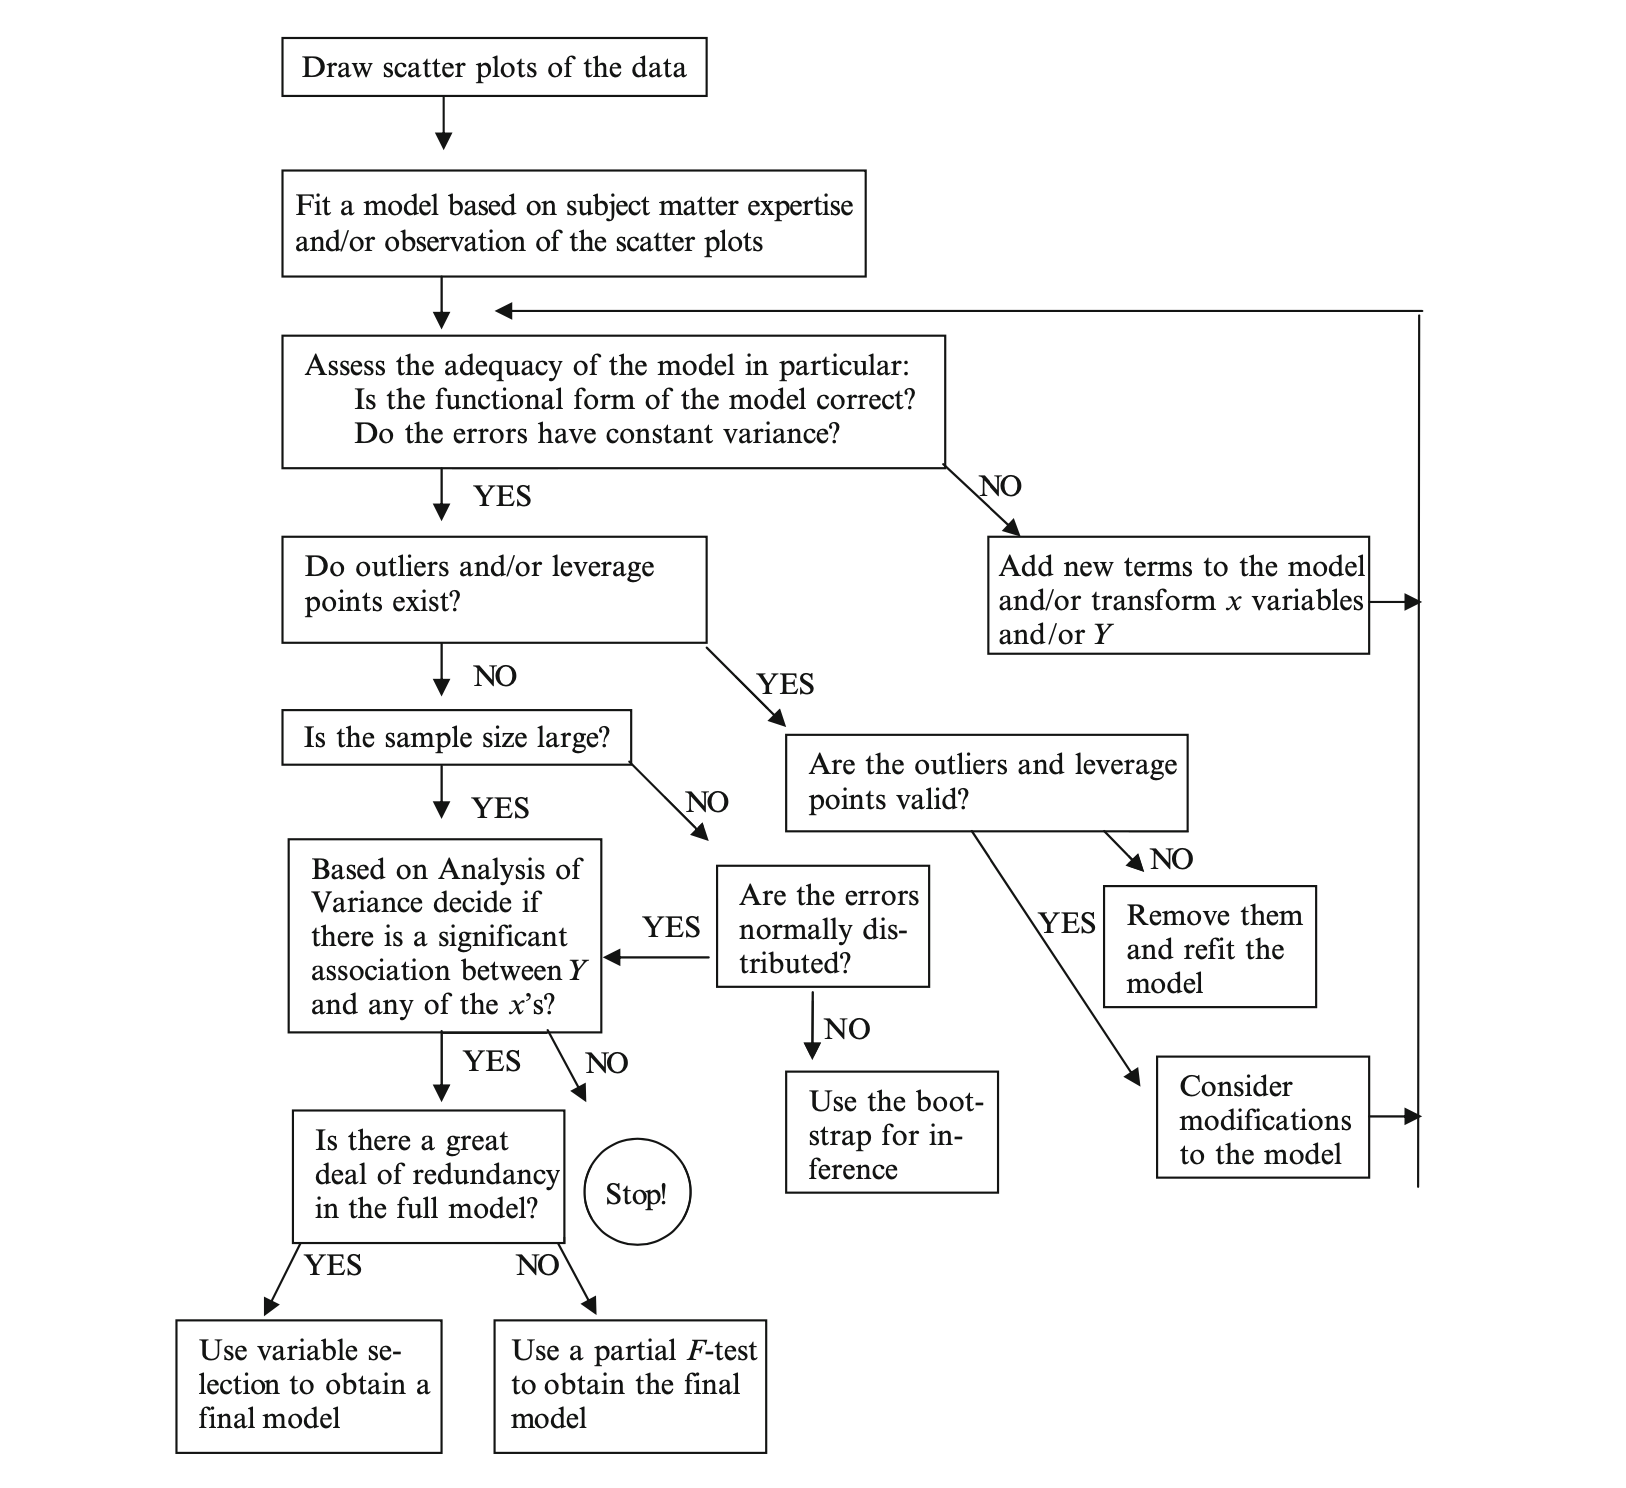
\includegraphics[width=\textwidth]{./images/data-analysis-flow}
%   \caption{Data Analysis Flow}
%   \label{data-analysis-flow}
% \end{figure}

\newpage

\section{Module 11 - Variable Selection}

\subsection{Variable Selection}

\textbf{What is the Goal?} \textit{Variable selection} or \textit{Prediction accuracy}
\textbf{What can occur?}
\begin{itemize}
  \item Overfitting: Too many predictors are in the ``final'' regression model.
  \item Underfitting: Not enough predictors are in the ``final'' regression model.
\end{itemize}
The \textit{bias-variance trade-off}: when we add more predictors to a valid model,
\begin{itemize}
  \item the bias of the predictions gets smaller ($\downarrow$)
  \item the variance of the estimated coefficients gets larger ($\uparrow$)
\end{itemize}

\subsubsection{Variable Selection: MLR and Likelihood-based Criteria}

Suppose that $yi, x_{1i}, x_{2i}, \dots, x_{pi}, i=1\dots n$ are observed values of Normal random variables, and

\begin{equation}
  y_i\>|\> x_{1i},\dots,x_{pi}\sim \mathcal{N}(\beta_0+ \beta_1x_{1i}+\dots+\beta_px_{pi}, \sigma^2),
\end{equation}

thus the \textbf{conditional density} of $y_i$ given $x_{1i},\dots,x_{pi}$ is given by

\begin{equation}
  f(y_i\>|\>x_{1i},x_{2i},\dots,x_{pi}) = \frac{1}{\sigma\sqrt{2\pi}}\exp\left( -\frac{(y_i - \{\beta_0+\beta_1x_{1i} + \dots + \beta_px_{pi}\})^2}{2\sigma^2} \right)
\end{equation}

\begin{definition}
  Assuming that the $n$ observations are independent, then the \textbf{likelihood function} of the unknown parameters $\beta_0,\beta_1,\dots,\beta_p,\sigma^2$ given $Y$ is given by
  \begin{align}
    L(\beta_0,\beta_1,\dots,\beta_p&,\sigma^2\>|\> Y)=\prod^n_{i=1} f(y_i\>|\> x_i)\\
    &=\prod^n_{n=1}\frac{1}{\sigma\sqrt{2\pi}}\exp\left( -\frac{(y_i - \{\beta_0+\beta_1x_{1i} + \dots + \beta_px_{pi}\})^2}{2\sigma^2}\right)\\
    &=\left(\frac{1}{\sigma\sqrt{2\pi}}\right)^n\exp\left( -\frac{1}{2\sigma^2}\sum^n_{i=1}(y_i - \{\beta_0+\beta_1x_{1i} + \dots + \beta_px_{pi}\})^2 \right)
  \end{align}
\end{definition}

\begin{definition}
  The \textbf{log-likelihood function} is given by
  \begin{gather}
    \log L(\beta_0,\beta_1,\dots,\beta_p,\sigma^2\>|\> Y)\\
    = -\frac{n}{2}\log(2\pi) - \frac{n}{2}\log(\sigma^2) - \frac{1}{2\sigma^2}\sum^n_{i = 1}(y_i - \{ \beta_0 + \beta_1x_{1i} + \dots + \beta_px_{pi}\})^2
  \end{gather}
\end{definition}
\begin{writenotes}
  Note that only the third term contains the regression parameters $\beta_0,\beta_1,\dots,\beta_p$, hence the MLEs of $\beta_0,\dots,\beta_p$ can be obtained by minimizing the third term only, which is equivalent to minimizing the residual sum of squares, RSS.

  Therefore, MLEs of $\beta_0,\dots,\beta_p$ are equal to the least square estimates.
\end{writenotes}

Substituting the LSEs of $\beta_0,\beta_1,\dots,\beta_p$, the \textbf{log-likelibood function} is re-written as

\begin{equation}\label{loglikelihood}
  \log L(\hat{\beta_0},\hat{\beta_1},\dots,\hat{\beta_p},\hat{\sigma}^2\>|\>Y) = -\frac{n}{2}\log(2\pi) - \frac{n}{2}\log(\sigma^2) - \frac{1}{2\sigma^2}RSS,
\end{equation}

where $RSS=\sum^n_{i=1} (y_i - \{\beta_0 + \beta_1x_{1i} + \dots + \beta_px_{pi} \})^2$

Solving for the MLE of $\sigma^2$, we obtain
\begin{equation}
  \sigma^2_{MLE} = \frac{RSS}{n}
\end{equation}

\begin{writenotes}
  Note that it differs slightly from the unbiased estimate of $\sigma^2$, namely, $S^2 = RSS / (n-p-1)$.
\end{writenotes}

Substituting the MLE of $\sigma^2$ into (\ref{loglikelihood}), we find that the likelihood associated with the maximum likelihood estimates is given by
\begin{align}
  \log L(\hat{\beta_0},\hat{\beta_1},\dots,\hat{\beta_p},\hat{\sigma}^2\>|\>Y) 
  &=\Bigg( -\frac{n}{2} \log(2\pi) - \frac{n}{2}\log\frac{RSS}{n} - \frac{1}{2}\left(\frac{RSS}{n}\right)(RSS)\Bigg)
  \\
  &= -\frac{n}{2}\log(2\pi) - \frac{n}{2}\log\left(\frac{RSS}{n}\right) - \frac{n}{2}\
\end{align}

\subsubsection{Akaike's Information Criterion (AIC)}

Akaike's Information Criterion is a likelihood-based criterion for assessing models, founded by Akaike (1973). It balances \textit{goodness} of fit and a penalty for model complexity.

\begin{definition}[AIC]
  \begin{align}
    AIC &= 2\left[ -\log L(\hat{\beta_0},\hat{\beta_1},\dots,\hat{\beta_p},\hat{\sigma}^2 \>|\> Y) + K \right]
    \\
  &=2\left(\frac{n}{2}\log(2\pi) + \frac{n}{2}\log\left( \frac{RSS}{n} \right) + \frac{n}{2} + K\right)\\
  &= n\log(2\pi) + n\log\left(\frac{RSS}{n}\right) + \frac{n}{2} + p + 4
  \end{align}
  where $K = p + 2$ is the number of parameters in the fitted model.
\end{definition}
\begin{writenotes}
  In R,
  \begin{equation}
    AIC = n\log\left(\frac{RSS}{n}\right) + 2p.
  \end{equation}
  Note that we dropped some terms by \textit{constant shift}.
\end{writenotes}

\begin{remark}
  The smaller the value of AIC, the better the model.
\end{remark}

When the sample size is small, or when the number of parameters estimated is a moderate to large fraction of the sample size, AIC tends to \textit{overfit} since the penalty for model complexity is NOT strong enough.

\begin{writenotes}
  For this reason, a \textit{bias corrected} verstion of AIC (Hurvich and Tsai, 1989) was developed.
\end{writenotes}

\subsubsection{Bayesian Information Criterion (BIC)}

\begin{definition}[BIC]
  \begin{align}
    BIC &= -2\log L(\hat{\beta_0},\hat{\beta_1},\dots,\hat{\beta_p},\hat{\sigma}^2\> | \> Y) + K\log(n)\\
    &= -2\left( -\frac{n}{2} \log(2\pi) - \frac{n}{2}\log\left(\frac{RSS}{n}\right) - \frac{n}{2} + K\log n \right)\\
    &= n\log(2\pi) + n\log\left(\frac{RSS}{n}\right) + n + p\log n + 2\log n
  \end{align}
  where $K = p + 2$ is the number of parameters in the fitted model.
\end{definition}
\begin{writenotes}
  In R:
  \begin{equation}
    BIC = n\log\left( \frac{RSS}{n} \right) + p\log(n).
  \end{equation}
\end{writenotes}

\begin{remark}
  The smaller the value of BIC, the better the model.
\end{remark}

When $n\geq 8,\log(n) > 2$, the penalty term in BIC is greater than that in AIC.

\begin{remark}
  BIC penalizes complex model more heavily than AIC, thus favours simpler models than AIC.
\end{remark}

\begin{remark}
Getting AIC, BIC in R:
\begin{verbatim}
  AIC(fittedmodel)
  BIC(fittedmodel)
  extractAIC(fittedmodel)
\end{verbatim}
\end{remark}


\subsubsection{A Model Selection Strategy}

\begin{enumerate}
  \item Calculate $R^2_{adj}$, AIC, corrected AIC, and BIC
  \item Compare the models which \textbf{minimize} AIC, corrected AIC, and BIC with the model that \textbf{maximizes} $R^2_{adj}$.
\end{enumerate}
Some notes...
\begin{itemize}
  \item The model with the lowest $MSE = S^2 = RSS / (n - p - 1)$ is equivalent to the model with the highest $R^2_{adj}$ among the same subset of predictors.
  \item Using $R^2_{adj}$ tends to over-fitting
  \item Consider $n:p$ ratio
\end{itemize}

\subsection{Stepwise Regression}

\subsubsection{Stepwise Methods}

Stepwise methods are automatic variable selection methods. If there are $p$ terms that can be added to the mean fucntion apart from the intercept, then there are $w^p$ possible regression equations

There are 3 stepwise algorithms: Backward, Forward, Stepwise.

\begin{algorithm}[Backward Elimination]
  \textbf{Backward Elimination} starts with all the potential terms in the model, then removes the term with the largest $p$-value each time to give a smaller information criterion.
\end{algorithm}

\begin{algorithm}[Forward Selection]
 The \textbf{Forward Selection} method is the \textit{reverse} of the backward method. It begins with no item in the model, then adds one term at a time (with the smallest $p$-value) until no further terms can be added to produce a smaller information criterion.
\end{algorithm}

\begin{algorithm}[Stepwise Regression]
  \textbf{Stepwise Regression} alternates forward steps with backward steps. At each stage, terms can be added, dropeed, or swapped.
\end{algorithm}

\begin{writenotes}
  Backward elimination and forward selection consider AT MOST $p + (p - 1) + \dots + 1 = \frac{p(p+1)}{2}$ of the $2^p$ possible predictor subsets, while stepwise regression can consider more subsets.

  The idea is to end up with a model where NO variables are redundant, given the other variables in the model. Often, backward elimination and forward selection will produce the same \textit{``final''} model.

  Backward elimination is often preferred to forward selection, since its initial estimate of $\sigma^2$ will usually be smaller.
\end{writenotes}

\subsubsection{Stepwise Regression: Cautions}

Selection \textbf{overstates} significance.
\begin{indentone}
  Estimates of regression coefficients are \textit{biased}

  $p$-values from $F$- and $t$- tests are generally smaller than their true values.
\end{indentone}

\begin{remark}[Forward and Backward in R]
The following illustrates R code for forward selection and backward elimination:
\begin{verbatim}
forwardAC <- step(interceptmodel, scope=list(lower=~1, upper=~X1+X2+X3))
backwardAC <- step(fullmodel, direction="backward", k=log(n))
\end{verbatim}
\end{remark}

\subsection{Penalized Linear Regression}

Penalized linear regression performs variable selection and regression coefficient estimation \textit{simutaneously}. It is a constrained least squares optimization problem

\begin{equation}
  \min_{\beta_0}\sum^n_{i=1}(Y_i - \VEC{\beta}'\VEC{x}_i)^2 + \sum^p_{j=1}p_\lambda(\cdot),
\end{equation}
where $p$ is the penalty function, and $\lambda\geq 0$ is the penalty parameter.

When $\lambda=0$, the solution is the least square estimates.

\begin{example}
  Some examples:
  \begin{itemize}
    \item Ridge Regression: $p_\lambda = \lambda\beta_j^2$
    \item LASSO Penalty: $p_\lambda = \lambda |\beta_j|$
    \item Adaptive LASSO
    \item SEAD
    \item Bridge Regression
    \item $\dots$
  \end{itemize}
\end{example}

\subsection{Cross Validation}

$k$-fold Cross-validation is a standard approach to assess the predictive ability of models ($y^*$) by evaluating their performance on a new data set.

\begin{algorithm}
Cross Validation steps
  \begin{enumerate}
    \item Divide the data (randomly) into $k$ (roughtly) equal sets.
    \item Stage A: Establish the model by using all but one of the $k$ folds; this set is called the \textbf{training data} set.
    \item Stage B: Use the remaining data set (the fold that was left out), called the \textbf{test data} to evaluate the model.
    \item Repeat Stages A \& B for $k$ times by changing the $k^\text{th}$ fold.
  \end{enumerate}
\end{algorithm}

\subsubsection{Cross Validation Prediction Error}

\newpage

\section{Appendix}

\subsection{Rules of Expectation}

\begin{itemize}
\item $\mathbb{E}(a) = a, a\in\R$
\item $\mathbb{E}(aY) = a\mathbb{E}(Y)$
\item $\mathbb{E}(X\pm Y) = \mathbb{E}(X) \pm \mathbb{E}(Y)$
\item $\mathbb{E}(XY) = \mathbb{E}(X)\mathbb{E}(Y)$
\item Tower Rule: $\mathbb{E}(Y) = \mathbb{E}[\mathbb{E}(Y\>|\>X)]$
\end{itemize}

  

\end{document}